\section{Introduction to Web Services}
(WHAT IS IMPORTANT HERE?)
The report and implementation will introduce the concepts of web services, by implementing the Travel Agency, TravelGood, and its underlying services utilized by the agency. These underlying services are provided by other organizations, LameDuck and NiceView. These organizations provides services for TravelGood using SOAP based web service. Furthermore, all three organizations use another service, FastMoney, which is a banking system provided as SOAP based web service. See \fref{fig:BlockDiagramOverView}

% \begin{figure}[h!]
%   \caption{A picture of a gull.}
%   \centering
%     \includegraphics[width=0.5\textwidth]{gull}
% \end{figure}

\begin{figure}[h!]
\centering
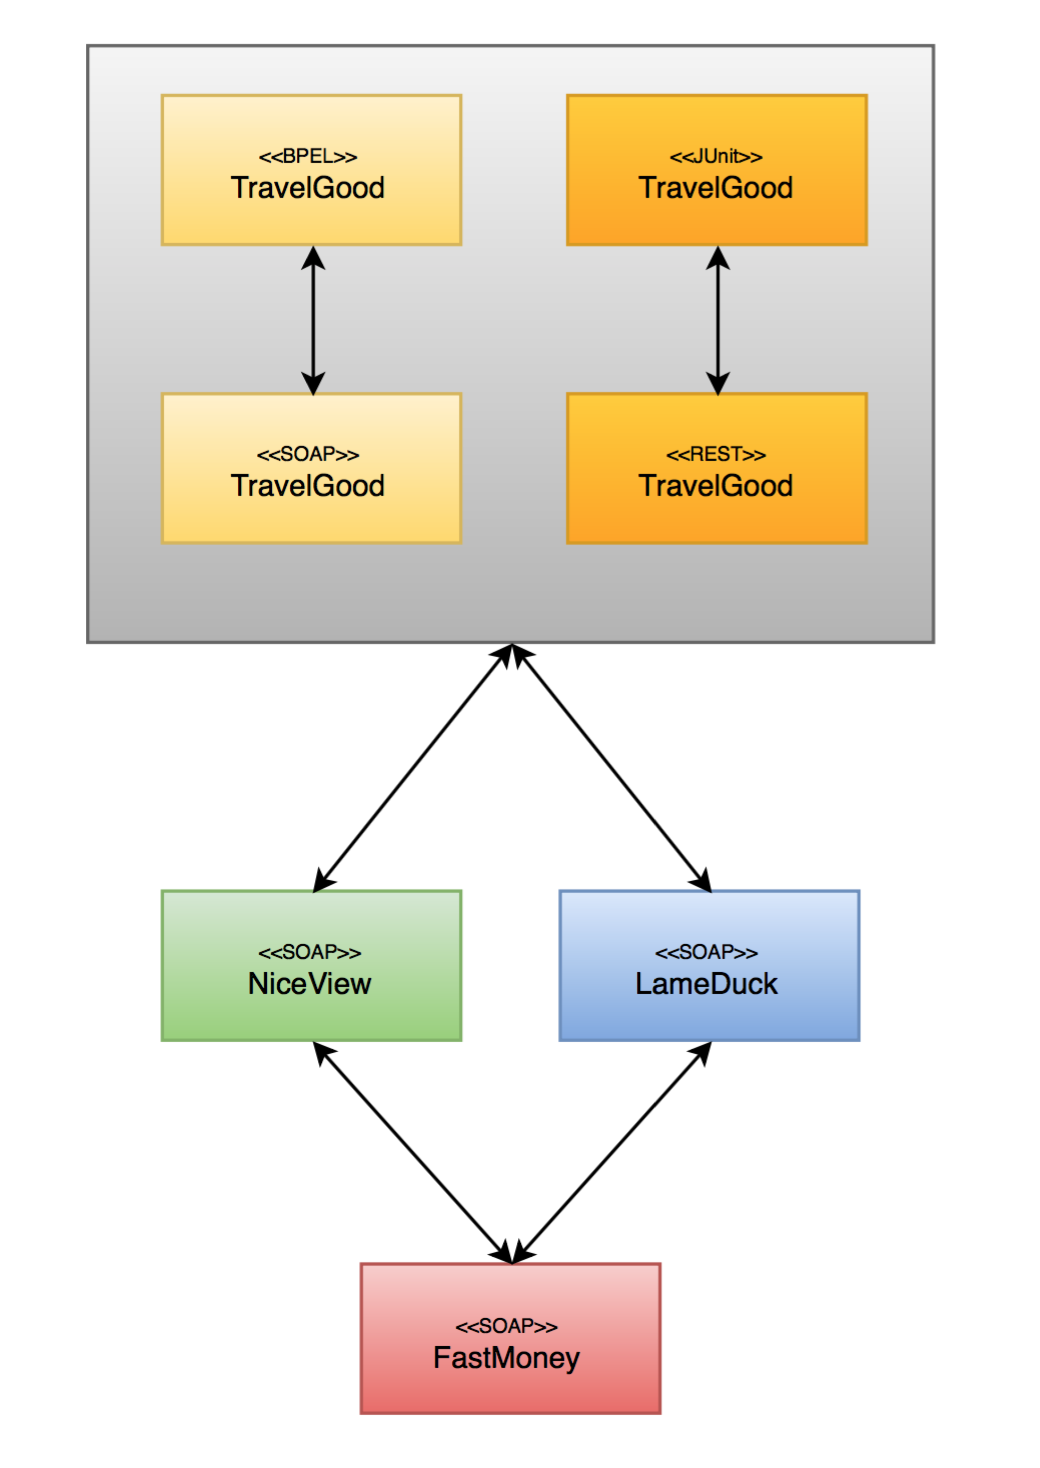
\includegraphics[width=0.4\textwidth]{Figures/BlockDiagramOverView.png}
\caption{Block Diagram - Overview}
\label{fig:BlockDiagramOverView}
\end{figure}

\subsection{Service Oriented Architecture}
\label{sub:Service Oriented Architecture}

The system utilizes SOA (Service Oriented Architecture) meaning that the systems contains several components that interacts with one another via a network using the Transport protocol, HTTP. The services are provided and described in a WSDL (Web Services Definition Language), defining the interfaces. Within the WSDL contains informations about the services/operations that can be invoked. Combined with all three services, they compose the Travel Agency service.

The Travel Agency will be implemented as both REST and SOAP based solutions, where the latter will be utilizing BPEL (Business Processing Execution Language), describing the processes that will be invoke services on NiceView and LameDuck.

\subsection{SOAP}
\label{sub:SOAP}
SOAP (Simple Object Access Protocol) is a protocol that describes how messages are exchanged on a network using HTTP as transport layer. These messages are based on XML (Extensible Markup Language) that has a set of defined rules on how these document are structured. Furthermore, a SOAP message also has a set of defined rules:

\begin{itemize}
  \item Header element that contains header information
  \item Body element that contains call and response information
  \item Fault element containing errors and status information
\end{itemize}

By being able to define the elements within a message, it introduces to strongly typed messages exchanged and messages can be sent/delivered reliably using WS-ReliableMessaging.

\subsection{BPEL}
\label{sub:BPEL}
With BPEL (Business Processing Execution Language) it is possible to describe the process of a business logic, and invoking services/operations on different web services, described in a WSDL. In another word, BPEL can be used to model the behavior of a use case, such as booking a hotel/flight.

\subsection{REST}
\label{sub:REST}
REST (Representational State Transfer) also uses HTTP protocol as its transport layer. Instead of using complex mechanism from other web services, such as SOAP, it uses simple operations from HTTP protocol that follows the CRUD (Create, Read, Update, Delete). Resources can then be accessed and execute several HTTP operations/verbs by knowing about the location of a resource in the form of URI.




% \subsection{Airline Reservation Service}
% \label{sub:Airline Reservation Service}
%
% The Airline Reservations Service, LameDuck, consists of three operations, Booking-, Cancel- and getFlights that are available for the TravelGood. LameDuck will retrieve all available flight informations from a given date. The list of informations will contain relevant informations such as departure and arrival time along with start airport and destination airport, its price and booking number.
%
% Booking of flight is handled by taking booking number and the credit card information from a given user, and upon doing so, it will validate the credit card information using FastMoney service to validate up against, for valid information and sufficient balance on the account.
%
% Lastly, cancellation is also possible in that it will cancel the booked flight, however full refund is not possible, instead a 50\% of the price will be refunded into the provided credit card information.
%
% \subsection{Hotel Reservation Service}
% \label{sub:Hotel Reservation Service}
%
% The Hotel Reservation Service, NiceView, will provide with three operations; Booking-, Cancel- and getHotels. With these operations, the service will retrieve hotel information from a given city and starting and ending date for accommodation. From these informations, NiceView will check if any rooms are available from the specified date and return a list of hotels containing available rooms and calculated price for each room.
%
% Booking of room for a given hotel is handled by taking booking number and credit card information. It checks for whether credit card is required to be validated, it will do so, calling the external web service, FastMoney.
%
% Lastly cancellation will cancel a booking by using a booking number.
%
% \subsection{Travel Agency}
% \label{sub:Travel Agency}
%
% The Travel Agency, TravelGood, will use NiceView and LameDuck and implement the business logic, as RESTful service and BPEL process. From TravelGood, it is possible to create an itinerary by booking flights and hotels for a given destination repeatedly and pay the whole itinerary by charging a credit card using FastMoney.
